\chapter{Making Tableasds}
\label{chp:chapter3}
\graphicspath{{figures/}{figures/chapter3/}}


\section{Making a Table}
An example \LaTeX\ table is shown below in Table~\ref{tab:comparison}.
You make a table by starting a table environment with a caption
and label.  You can specify the text that shows up in the Table of
Contents using the optional parameter box, [], that's at the
beginning of the $\backslash$caption command. You tell the table how
many columns in the beginning of the tabular environment using a
command like this: $|$ l $|$ c $|$ r $|$. That would create a table with 3 columns
that are left-aligned, centered and right-aligned, in that order. The $|$'s tell \LaTeX\ that
you want bars separating the columns. Of course, you can also make tables without the $|$ characters, in which case no lines will be added between the fields, which often looks better. You can also add horizontal
lines using the $\backslash$hline command. This example is also centered in the page using the
$\backslash$centering command.
%
\begin{table}[b]
\centering
\savebox{\tempbox}{
%
\begin{tabular}{|l|c|c|r|}
\hline

Table Name  & Column 2 & Column 3   & Column 4 \\
\hline
First Row   & 4780286  & 72.941376  & A \\
Second Row  & 4069335  & 62.093124  & B \\
Third Row   & 4074900  & 62.178040  & C \\
\hline
Fourth Row  & 4000000  & 60.000000  & Z \\
\hline

\end{tabular}}
% set width
\ifdim\wd\tempbox<\TPTminimum\relax \tempwidth=\TPTminimum\relax
\else\tempwidth=\wd\tempbox
\fi
% format
\begin{minipage}{\tempwidth}\centering
\caption[Example table]{Description of the table, where the caption is long enough to go onto more than one line. The table caption should not extend beyond the edges of the table, and should make an ``inverted pyramid.''}
\label{tab:comparison}
\usebox{\tempbox}
%\end{threeparttable}
\end{minipage}
\end{table}
%

Landscape tables can also be inserted, if desired, using the \verb-sidewaystable- environment, which is defined in the \verb!rotating! package. An example is found on the next page, in Table~\ref{tab:landscape}. Note that landscape tables and figures should be the exception rather than the rule, since they are more awkward to read. However, if you have an especially wide table or figure that cannot be reduced in size without losing required resolution, placing it in landscape may be a good idea.
\begin{sidewaystable}
\centering
\savebox{\tempbox}{
\setlength{\tabcolsep}{6mm}
\begin{tabular}{lcccc}
Year & Method of CVD Deposition & Thickness ($\mu$m) & Hardness (MPa) & Resistivity ($\Omega\cdot$m)\\ 
\hline\\[-11pt]
1999 & LPCVD & 5.1 & 175 & 2.3$\times10^{-5}$\\
2000 & PECVD & 17.2 & 101& 1.5$\times10^{-5}$\\
2002 & PECVD & 4.3 & 55 & 3.4$\times10^{-5}$\\
2004 & LPCVD & 1.1 & 225 & 5.1$\times10^{-5}$\\
\hline
\end{tabular}}
% set width
\ifdim\wd\tempbox<\TPTminimum\relax \tempwidth=\TPTminimum\relax
\else\tempwidth=\wd\tempbox
\fi
% format
\begin{minipage}{\tempwidth}\centering
\caption{A landscape table}\vspace*{6pt}
\label{tab:landscape}
\usebox{\tempbox}
%\end{threeparttable}
\end{minipage}
\end{sidewaystable}


\subsection{First Subsection}
Also into subsections.

\subsection{Second Subsection}
Which really helps organization and automatically gets added to the Table
of Contents and gets linked to by the hyperref package.

\section{Citation Example}
One of the greatest parts about \LaTeX\ is BibTeX. You can just call
the $\backslash$cite command and it will organize the whole references section for you as long as there is an entry in the refs.bib file (or whichever other .bib file you tell it to use; see the source for master.tex).
Here is an example of citing previous works
\cite{guy06best,guy06second}.

\section{Fixed Width Figure Example} \label{sec:intro_figure_example}
This part also shows how to include a basic figure like the ones
shown in Figures~\ref{fig:intro_stuff2} and \ref{fig:intro_stuff}. %Figure~\ref{fig:example} illustrates the use of a figure placed in landscape.
\begin{figure}[t]
  \centering
  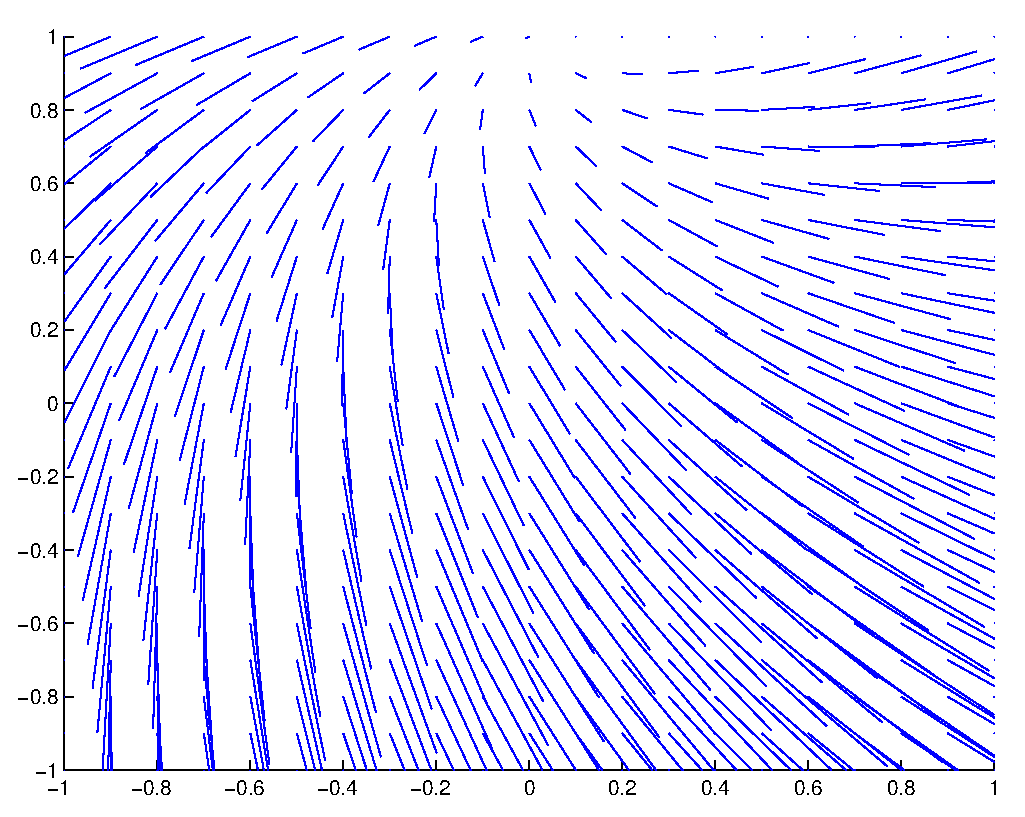
\includegraphics[width = 2in]{stuff}
  \caption[Example small width figure]{
Example small width figure, showing how to use the width option.}
%
  \label{fig:intro_stuff2}
\end{figure}

\begin{figure}[t]
  \centering
  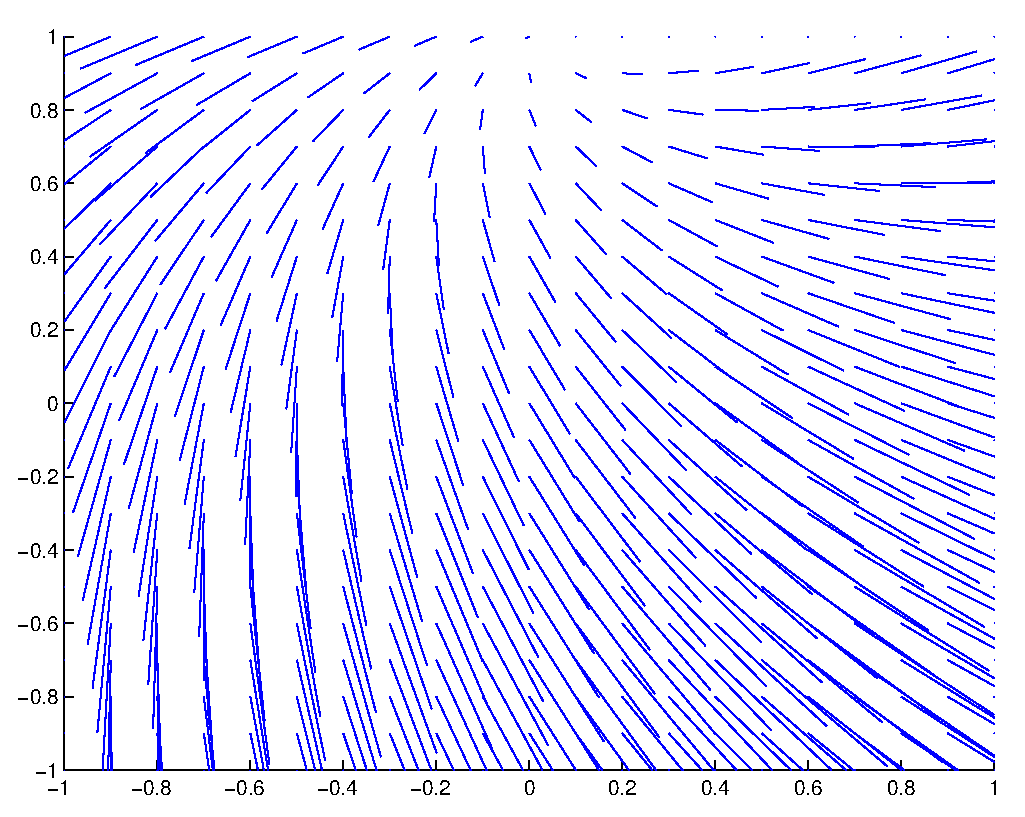
\includegraphics[width=5.5in]{stuff}
  \caption[Example fixed width figure]{
This figure is just a simple figure with a width set at 5.5~in. An example of a
figure whose size depends on the width of the page is given in
Figure \ref{fig:appendix_some_pic} in Section~\ref{sec:appendixa_figure_example} of Appendix~\ref{apdx:appendixa}.}
%
  \label{fig:intro_stuff}
\end{figure}

%\begin{sidewaysfigure}[p]
%\includegraphics[scale=0.8]{examplegraphic}
%\caption{An example of a landscape graphic.}
%\label{fig:example}
%\end{sidewaysfigure}

\section{Math and Equation Example, Where the Heading Is Made so Long That It Extends onto a Second Line}
Here is how to use inline math mode to define lambda like this,
$\lambda$, and how to declare Equations~\eqref{eqn:definition_Ix}
and~\eqref{eqn:definition_Iy}

\begin{equation} \label{eqn:definition_Ix}
I_x(x,y) = \pd{I(x,y)}{x},
\end{equation}

\begin{equation}\label{eqn:definition_Iy}
I_y(x,y) = \pd{I(x,y)}{y}.
\end{equation}

 Or you can create equation arrays like
\begin{align}
  \alpha &= \beta^\gamma \\
  x &= \frac{1}{\alpha} \label{eq:cool_1} \\
  y &= \sqrt{\abs{\frac{\gamma}{\beta}}}  \\
  \zeta &= x^y \label{eq:cool_2}.
\end{align}


The lines in the array can be referenced by saying things like: In
Eqn.~\eqref{eq:cool_1} we show a wonderful equation, but it's not nearly as
amazing as Eqn.~\eqref{eq:cool_2}.
